\input{macros_td.tex}


\begin{document}
\feuille {1} 
%\vspace*{1cm}

\exos
\textbf{Objectifs :}
\begin{itemize}
	\item Manipulation de flux (d'images en l'occurence)
	\item Mise en \oe uvre d'algorithmes de traitement d'images
	\item Utilisation de Collection : List ; Comparaison LinkedList ? ArrayList
\end{itemize}

\textbf{Pr�-requis :}\\
Pour manipuler les images, on utilisera la classe BufferedImage, voir sur l'API Java :\\
http://docs.oracle.com/javase/7/docs/api/java/awt/image/BufferedImage.html

\begin{figure}[h]
\centerline{
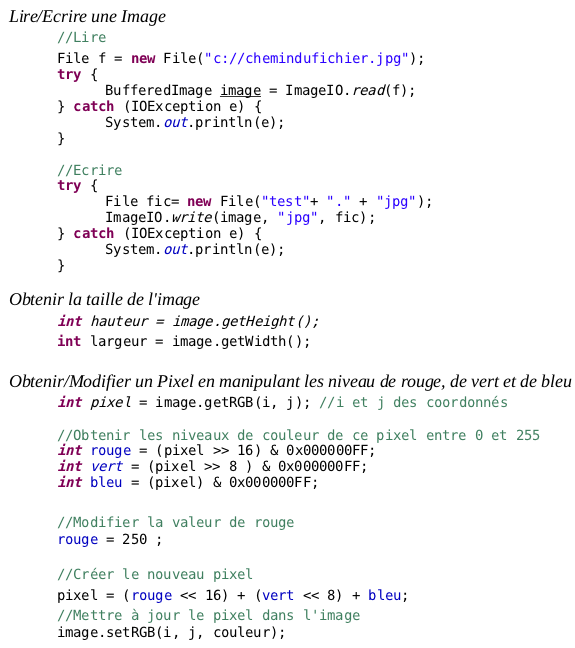
\includegraphics[scale=0.6]{image}}
\label{fig:une}
\end{figure}


\exos
\begin{enumerate}
\item Ecrire un main qui lit un fichier image "image.jpg" et en fait une copie
nomm�e "image\_copie.jpg"
\item Cr�er les classes {\tt Pixel} et {\tt ImageATraiter}.
La classe {\tt Pixel} poss�de des attributs $rouge$, $bleu$ et $vert$ de type entier.
La classe {\tt ImageATraiter} contient une {\tt List} de {\tt Pixel}.
\item Ecrire dans la classe {\tt ImageATraiter} la m�thode
\textit{public void obtainPixelFromImage(BufferedImage image)}
qui prend une {\tt BufferedImage} en param�tre et stocke chacun de ses pixels dans la
liste.

\item Ecrire dans la classe {\tt Pixel} une m�thode qui retourne le niveau de gris du pixel.
Pour calculer le niveau de gris, on utilisera la formule :
0.299*rouge + 0.587*vert + 0.114*bleu

\item Ecrire dans {\tt ImageATraiter} la m�thode
\textit{public void setNEtB(BufferedImage image)}
qui prend en param�tre une {\tt BufferedImage}, stocke tous ses pixels dans la liste, puis
modifie chacun des pixels de l'image en les transformant en noir et blanc. Pour
transformer un pixel en noir et blanc, on fait rouge=bleu=vert=niveau de gris.
\item Tester cette m�thode en �crivant un main qui obtient une {\tt BufferedImage} du disque
dur, la transforme en noir et blanc, puis l'�crit sur le disque dur.
Comparer l'efficacit� de l'algorithme en impl�mentant la solution avec {\tt ArrayList} puis
{\tt LinkedList} dans la classe {\tt ImageATraiter}. Que constatez vous ?
\item Impl�menter l'algorithme de $Sobel$ qui permet de ne conserver que les contours d'une
image dont voici une version simplifi�e :
\begin{verbatim}
Pour i de 0 � largeur de image
    Pour j de 0 � hauteur de image
       sum_r=rouge(pixel(j+1, i-1)) + rouge(pixel(j+1, i)) +
       rouge(pixel(j+1, i+1)) -
       (rouge(pixel(j-1, i-1)) + rouge(pixel(j-1, i)) +
       rouge(pixel(j-1, i+1)))
       sum_b=bleu(pixel(j+1, i-1)) + bleu(pixel(j+1, i)) +
       bleu(pixel(j+1, i+1)) -
       (bleu(pixel(j-1, i-1)) + bleu(pixel(j-1, i)) +
       bleu(pixel(j-1, i+1)))
       sum_v=vert(pixel(j+1, i-1)) + vert(pixel(j+1, i)) +
       vert(pixel(j+1, i+1)) -
       (vert(pixel(j-1, i-1)) + vert(pixel(j-1, i)) +
       vert(pixel(j-1, i+1)))
       pixel(j, i) = (0.299*sum_r + 0.587*sum_g + 0.114*sum_b))
\end{verbatim}

\end{enumerate}
 
%\end{figure}
 \end{document}